\documentclass[aspectratio=169]{beamer}
\usepackage[utf8]{inputenc} % codificacao de caracteres
\usepackage[T1]{fontenc}    % codificacao de fontes
\usepackage[english]{babel}  % idioma
\usepackage{graphics,amssymb,amsfonts,amsmath}
\usepackage{tikz}
\usepackage{enumerate,hyperref}
\usepackage{palatino}	% Fonte sem serifa
\usepackage{ragged2e}	% Paragrafo justificado
%\usepackage{minted}	% Highlight para codigos de programacao
\usepackage{booktabs} % tabelas
\usepackage{multicol}
\usepackage{multirow}

%\usepackage[table]{xcolor}


% Veja mais temas e cores em http://www.hartwork.org/beamer-theme-matrix/
\usetheme{Montpellier}         % tema
\usecolortheme{orchid}      % cores
\usefonttheme[onlymath]{serif} % fonte modo matematico
% Colocando numero de paginas no slide
\setbeamertemplate{footline}[frame number]



\DeclareGraphicsExtensions{.pdf,.JPG,.png} % compilamos apenas com pdflatex
%\graphicspath{{./figuras/}} % caminho onde as figuras estarao disponiveis


\graphicspath{{figuras/}}

% ---------------------------------------------------------------------------- %
% T�tulo                                                                       %
% ---------------------------------------------------------------------------- %

\title[\sc{Teoria de Circuitos Eletrônicos 1}]{\LARGE Aula 8 - Energy Storage Elements}
\author[Prof. Marcelino Andrade]{Prof. Marcelino Andrade}
\institute{Faculdade UnB Gama} % opcional
\date{\today}

\begin{document}
\justifying % Paragrafo justificado
\pagebreak

\begin{frame}
  \titlepage
\end{frame}


% ----------------- NOVO SLIDE --------------------------------
\begin{frame}{Contents}

\tableofcontents
%\begin{center}	
     		Introduction to Electric Circuits by James A. Svoboda, Richard C. Dorf, 9th Edition 
  %   		Fundamentals of Electric Circuits by Alexander and Sadiku, 4th Edition	
%\end{center}	
\end{frame}

% ----------------- NOVA SECÇÂO -----------------------------
\section{Introduction (7.1)}
% ----------------- NOVO SLIDE --------------------------------
\begin{frame}[fragile]
	\frametitle{Introduction}
		\begin{tabular}{cc}
			\begin{columns}
				\begin{column}{1\textwidth}  %%<--- here
					This chapter introduces two more circuit elements, the capacitor and the inductor. Consequently:	
		
					\begin{itemize}
						\item[$\clubsuit$]{Electric circuits that contain capacitors and/or inductors are represented by differential equations, able to store energy and have memory;}
						\item[$\clubsuit$]{In a dc circuit, capacitors act like open circuits, and inductors act like short circuits;}
						\item[$\clubsuit$]{Series or parallel capacitors and inductors can be reduced to an equivalent capacitor and equivalent inductor, respectively;}	
						\item[$\clubsuit$]{An op amp and a capacitor and/or inductors can be used to make circuits that perform the mathematical operations of
integration or differentiation.;}	
					\end{itemize}
					
				\end{column}
			\end{columns}
		
	\end{tabular}
\end{frame}

% ----------------- NOVA SECÇÂO -----------------------------
\section{Capacitors (7.2) and Inductors (7.5)}
% ----------------- NOVO SLIDE --------------------------------
\begin{frame}[fragile]
\frametitle{Capacitors}
\begin{columns}
\begin{column}{1\textwidth}  %%<--- here
\textbf{Capacitance} is a measure of the ability of a device to store energy in the form of an electric field.
\end{column}
\end{columns}

	

	\begin{columns}
		\begin{column}{.2\textwidth}  %%<--- here
		\begin{center}
			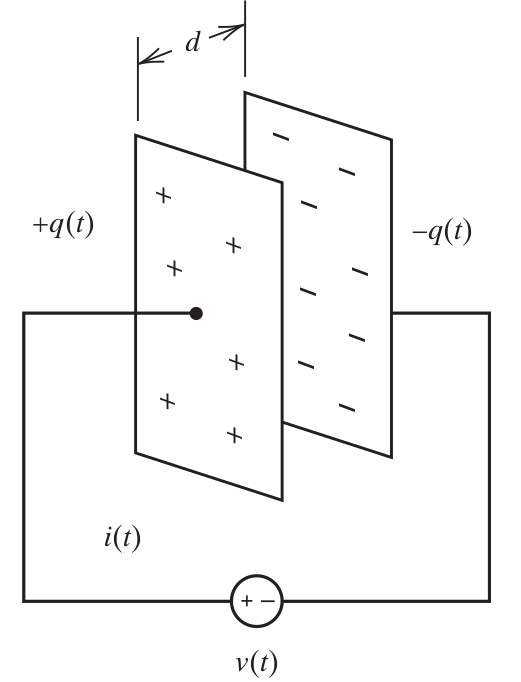
\includegraphics[height=3.5cm]{figura1.png}
		\end{center}
		\end{column}
		\begin{column}{.22\textwidth}  %%<--- here
		\begin{center}
			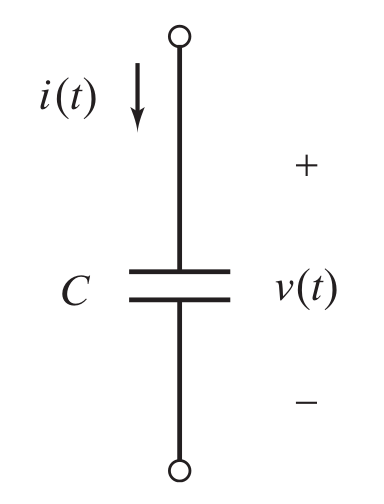
\includegraphics[height=3cm]{figura2.png}
		\end{center}
		\end{column}
		\begin{column}{.17\textwidth}  %%<--- here
		\begin{center}
			\scriptsize	\begin{equation} 
					 {C=\epsilon \frac{A}{d}} 
					\end{equation}
			\scriptsize	\begin{equation} 
					C=\frac{q(t)}{v(t)}
					\end{equation}\\
		    \scriptsize	\begin{equation} 
					i(t)=\frac{d}{dt}q(t)
					\end{equation}			
		\end{center}
		\end{column}

		\begin{column}{.25\textwidth}  %%<--- here
		\begin{center}
		

		\scriptsize	\begin{equation} 
				i(t)=C\frac{d}{dt}v(t)
				\end{equation}
		\scriptsize	\begin{equation} 
				v(t)=\frac{1}{C}\int_{-\infty}^{t} i(\tau) d\tau
				\end{equation}\\
		\tiny	\flushleft	\scalebox{0.7}{$C$ = capacitance},\
					\scalebox{0.7}{$A$ = area},\
					\scalebox{0.7}{$d$ = distance},\
					\scalebox{0.7}{$q$ = electric charge},\
					\scalebox{0.7}{$v$ = voltage,} \
					\scalebox{0.7}{$i$ = current,} \
					\scalebox{0.7}{$\epsilon$ = dielectric constant}.\
										
		\end{center}
		\end{column}
	\end{columns} 	
	

	\begin{columns}
		\begin{column}{.2\textwidth}  %%<--- here
		\begin{center}
		\textbf{\scalebox{0.55}{Typical capacitor}}
		\end{center}
		\end{column}
		\begin{column}{.22\textwidth}  %%<--- here
		\begin{center}
		\textbf{\scalebox{0.55}{Symbol for capacitor}}	
		\end{center}
		\end{column}
		\begin{column}{.48\textwidth}  %%<--- here
		\begin{center}
		\textbf{\scalebox{0.55}{Capacitor equations}}
		\end{center}
		\end{column}
%		\begin{column}{.2\textwidth}  %%<--- here
%		\begin{center}
%		\textbf{\scalebox{0.55}{Capacitor equations}}	
%		\end{center}
%		\end{column}
	\end{columns} 	

	

\end{frame}
% ----------------- NOVO SLIDE --------------------------------
\begin{frame}[fragile]
\frametitle{Inductors}
\begin{columns}
\begin{column}{1\textwidth}  %%<--- here
\textbf{Inductance} is a measure of the ability of a device to store energy in the form of a magnetic field.
\end{column}
\end{columns}
	
	\begin{columns}
		\begin{column}{.2\textwidth}  %%<--- here
		\begin{center}
			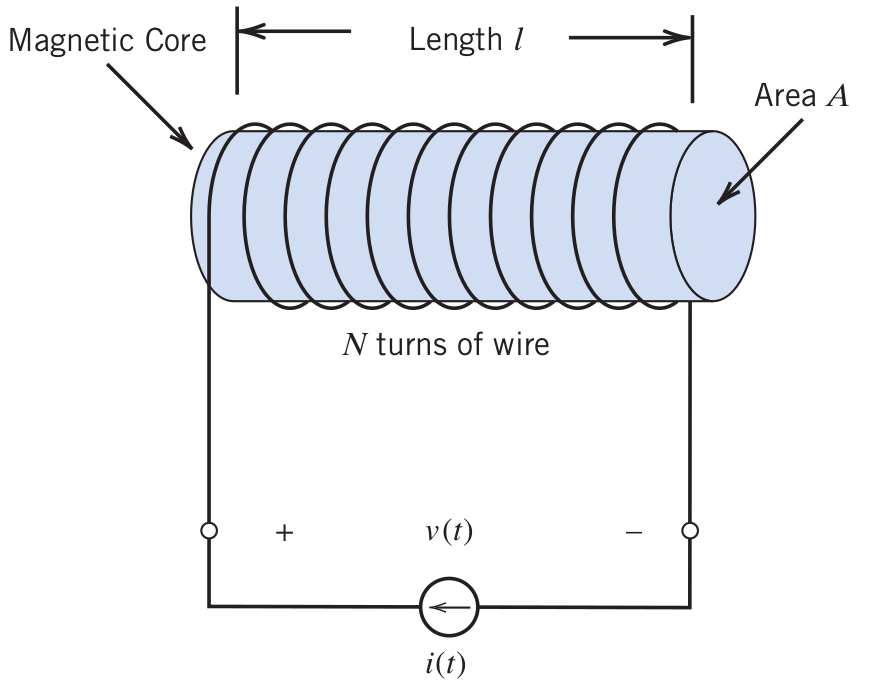
\includegraphics[height=2.7cm]{figura3.png}
		\end{center}
		\end{column}
		\begin{column}{.22\textwidth}  %%<--- here
		\begin{center}
			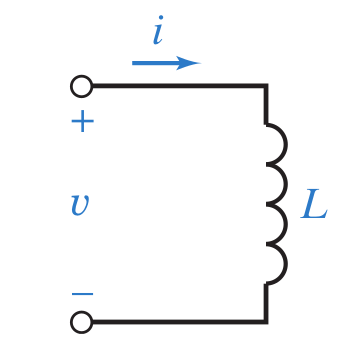
\includegraphics[height=2.7cm]{figura4.png}
		\end{center}
		\end{column}
		\begin{column}{.17\textwidth}  %%<--- here
		\begin{center}
			\scriptsize	\begin{equation} 
					  {L=\mu \frac{N^{2}A}{l}}
					\end{equation}
			\scriptsize	\begin{equation} 
					L=\frac{\phi(t)}{i(t)}
					\end{equation}\\
		    \scriptsize	\begin{equation} 
					v(t)=\frac{d}{dt}\phi(t)
					\end{equation}			
		\end{center}
		\end{column}

		\begin{column}{.25\textwidth}  %%<--- here
		\begin{center}
		

			\scriptsize	\begin{equation} 
					  v(t)=L\frac{d}{dt}i(t)
					\end{equation}
			\scriptsize	\begin{equation} 
					i(t)=\frac{1}{L}\int_{-\infty}^{t} v(\tau) d\tau
					\end{equation}\\
		\tiny	\flushleft	\scalebox{0.7}{$L$ = indutance},\
					\scalebox{0.7}{$A$ = area},\	
					\scalebox{0.7}{$\mu$ = permeability},\
					\scalebox{0.7}{$l$ = length of the winding},\
					\scalebox{0.7}{$N$ = number of turns,} \
					\scalebox{0.7}{$\phi$ = fluxo magnético,}\
					\scalebox{0.7}{$v$ = voltage,} \
					\scalebox{0.7}{$i$ = current,} \


										
		\end{center}
		\end{column}
	\end{columns} 	
	

	\begin{columns}
		\begin{column}{.2\textwidth}  %%<--- here
		\begin{center}
		\textbf{\scalebox{0.55}{Typical inductor}}
		\end{center}
		\end{column}
		\begin{column}{.22\textwidth}  %%<--- here
		\begin{center}
		\textbf{\scalebox{0.55}{Symbol for inductor}}	
		\end{center}
		\end{column}
		\begin{column}{.48\textwidth}  %%<--- here
		\begin{center}
		\textbf{\scalebox{0.55}{Inductor equations}}
		\end{center}
		\end{column}
%		\begin{column}{.2\textwidth}  %%<--- here
%		\begin{center}
%		\textbf{\scalebox{0.55}{Capacitor equations}}	
%		\end{center}
%		\end{column}
	\end{columns} 	

	
	

\end{frame}
% ----------------- NOVO SLIDE --------------------------------
\begin{frame}[fragile]
\frametitle{Capacitors}
	
	\begin{tabular}{r}
	
	\begin{columns}
		\begin{column}{1\textwidth}  %%<--- here
	The voltage across a \textbf{capacitor} cannot change instantaneously.
		\end{column}
	\end{columns}\\
		\begin{columns}
		\begin{column}{.25\textwidth}  %%<--- here
%		  \begin{center}
		  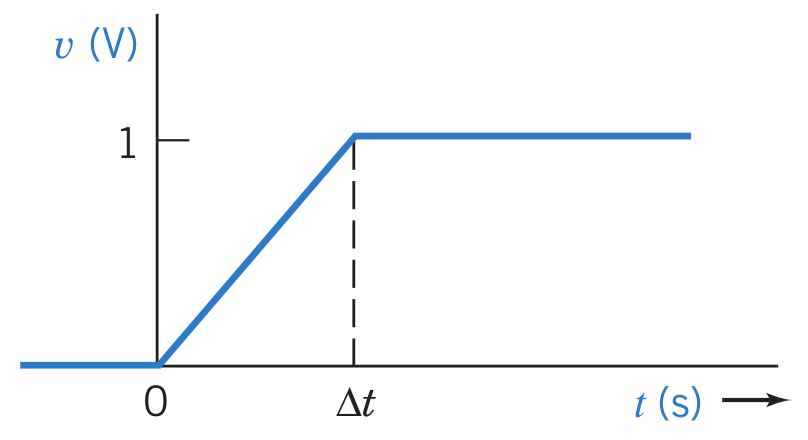
\includegraphics[height=2cm]{figura5.png}     			
%		  \end{center}
		\end{column}

		\begin{column}{.1\textwidth}  %%<--- here
%		  \begin{center}
		 $$i(t)=C\frac{d}{dt}v(t)$$     			
%		  \end{center}
		\end{column}
		
		
		
		\begin{column}{.3\textwidth}  %%<--- here
%		\begin{center}		
		    $$
	    i(t)=
	    \begin{cases}
	    0, \  t<0 \\
	    \\
	    \frac{C}{\Delta t}, \ 0 \leq \ t \leq \Delta t\\
	    \\
	    0,\ t>\Delta t
	    \end{cases}
	    $$ 			
%		\end{center}

		\end{column}
		
		
	\end{columns}\\
	
		\begin{columns}
		\begin{column}{1\textwidth}  %%<--- here
	\newline 
Clearly, $\Delta t$ cannot decline to zero or we would experience an infinite current. An infinite current is an
impossibility because it would require infinite power. Thus, an instantaneous $(\Delta t =0)$ change of
voltage across the capacitor is not possible. In other words, we cannot have a discontinuity in $v(t)$.
		\end{column}
	\end{columns}\\
	
\end{tabular}
	
\end{frame}


% ----------------- NOVO SLIDE --------------------------------
\begin{frame}[fragile]
\frametitle{Inductors}
	
	\begin{tabular}{r}
	
	\begin{columns}
		\begin{column}{1\textwidth}  %%<--- here
	The current in an \textbf{inductance} cannot change instantaneously.
		\end{column}
	\end{columns}\\
		\begin{columns}
		\begin{column}{.25\textwidth}  %%<--- here
%		  \begin{center}
		  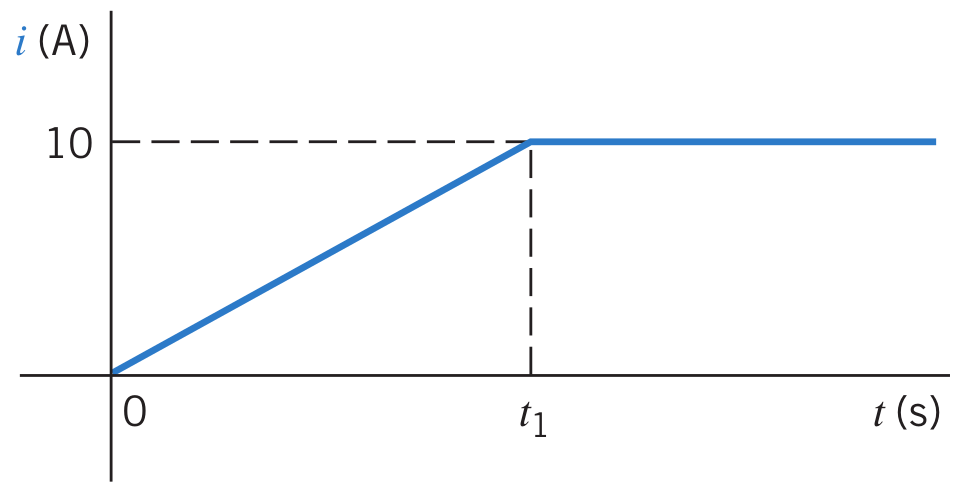
\includegraphics[height=2cm]{figura6.png}     			
%		  \end{center}
		\end{column}

		\begin{column}{.1\textwidth}  %%<--- here
%		  \begin{center}
		 $$  v(t)=L\frac{d}{dt}i(t)$$\\
		\tiny $L=0.1\ H$
%		  \end{center}
		\end{column}
		
		
		
		\begin{column}{.3\textwidth}  %%<--- here
%		\begin{center}		
		    $$
	    i(t)=
	    \begin{cases}
	    0, \  t<0 \\
	    \\
	    \frac{1}{t_{1}}, \ 0 \leq \ t_{1} \leq \Delta t\\
	    \\
	    0,\ t>t_{1}
	    \end{cases}
	    $$ 			
%		\end{center}

		\end{column}
		
		
	\end{columns}\\
	
		\begin{columns}
		\begin{column}{1\textwidth}  %%<--- here
	\newline 
Clearly, we cannot let $t_{1}=0$ because the voltage required would
then become infinite, and we would require infinite power at the terminals of the inductor. Thus,
instantaneous changes in the current through an inductor are not possible. In other words, we cannot have a discontinuity in $i(t)$.
		\end{column}
	\end{columns}\\
	
\end{tabular}
	
\end{frame}

% ----------------- NOVO SLIDE --------------------------------
\begin{frame}[fragile]
\frametitle{Capacitors, Inductors and \textbf{initial condition}}
	
	\begin{tabular}{r}
	
	\begin{columns}
		\begin{column}{.5\textwidth}  %%<--- here
	\textbf{Capacitors: \newline} 
		\end{column}
		\begin{column}{.5\textwidth}  %%<--- here
	 \textbf{Inductors: \newline} 
		\end{column}
	\end{columns}\\
		\begin{columns}
		\begin{column}{.5\textwidth}  %%<--- here
%		\begin{center}	
\scriptsize This equation says that the capacitor voltage $v(t)$ can be found by integrating the capacitor current from
time $-\infty$ until time $t$.\\
$$v(t)=\frac{1}{C}\int_{-\infty}^{t} i(\tau) d\tau$$\\
$$v(t)=\frac{1}{C}\int_{t_{0}}^{t} i(\tau) d\tau+\frac{1}{C}\int_{-\infty}^{t_{0}} i(\tau) d\tau$$\\
$$v(t)=\frac{1}{C}\int_{t_{0}}^{t} i(\tau) d\tau+v(t_{0})$$\\
The time $t_{0}$ is called the \textbf{initial time}, and the capacitor voltage $v(t_{0})$ is called the \textbf{initial condition}.
%		\end{center}

		\end{column}
		
		\begin{column}{.5\textwidth}  %%<--- here
%		\begin{center}		
		\scriptsize This equation says that the inductor current $i(t)$ can be found by integrating the inductor voltage from
time $-\infty$ until time $t$.\\
$$i(t)=\frac{1}{L}\int_{-\infty}^{t} v(\tau) d\tau$$\\
$$i(t)=\frac{1}{L}\int_{t_{0}}^{t} v(\tau) d\tau+\frac{1}{L}\int_{-\infty}^{t_{0}} v(\tau) d\tau$$\\
$$i(t)=\frac{1}{L}\int_{t_{0}}^{t} v(\tau) d\tau+i(t_{0})$$\\
The time $t_{0}$ is called the \textbf{initial time}, and the inductor current $i(t_{0})$ is called the \textbf{initial condition}.
%		\end{center}

		\end{column}
		
		
	\end{columns}\\
	

	
\end{tabular}
	
\end{frame}



% ----------------- NOVO SLIDE --------------------------------
\begin{frame}[fragile]
\frametitle{Capacitor Current and Voltage}
\begin{tabular}{r}
	    \begin{columns}
		\begin{column}{1\textwidth}
		\textbf{EXAMPLE 7.2-1} - Find the current for a capacitor $C = 1mF$ when the voltage across
the capacitor is represented by the signal shown in Figure below. \\
		\end{column}
	  \end{columns}\\
		\begin{columns}
		  \begin{column}{.7\textwidth}  %%<--- here
		    \begin{center}
    	  		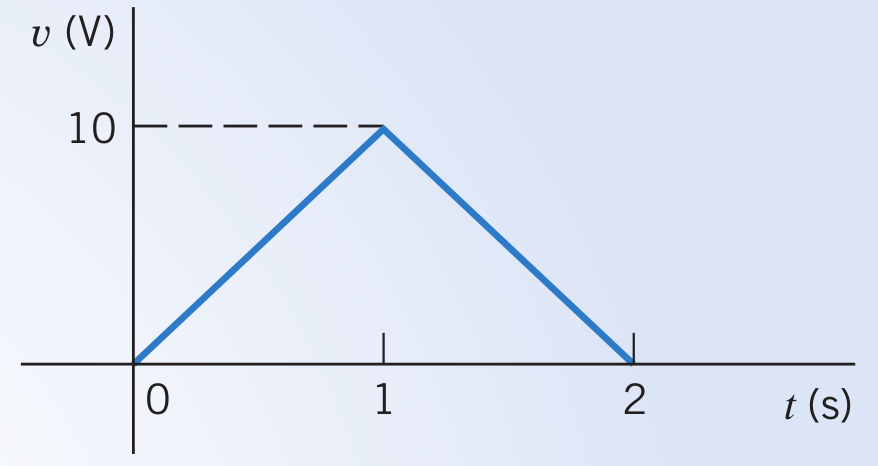
\includegraphics[height=.4\textwidth]{figura7.png}	
		    \end{center}
		\end{column}
		
	 
	
	
	
	\end{columns}
	

	
\end{tabular}
\end{frame}




% ----------------- NOVO SLIDE --------------------------------
\begin{frame}[fragile]
\frametitle{Inductor Current and Voltage}
\begin{tabular}{r}
	    \begin{columns}
		\begin{column}{1\textwidth}
		\textbf{EXAMPLE 7.5-2} - Figure below shows a circuit together with two plots. The plots represent the current and voltage of the inductor in
the circuit. Determine the value of the inductance of the inductor. \newline\\
		\end{column}
	  \end{columns}\\
		\begin{columns}
		  \begin{column}{.3\textwidth}  %%<--- here
		    \begin{center}
    	  		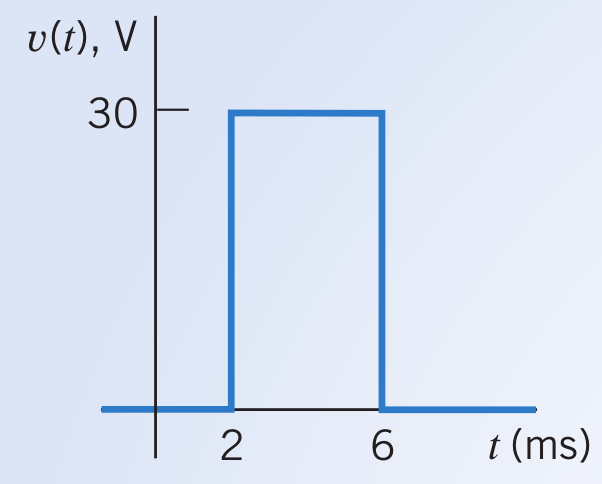
\includegraphics[height=.7\textwidth]{figura8.png}	
		    \end{center}
		\end{column}
		

		  \begin{column}{.3\textwidth}  %%<--- here
		    \begin{center}
    	  		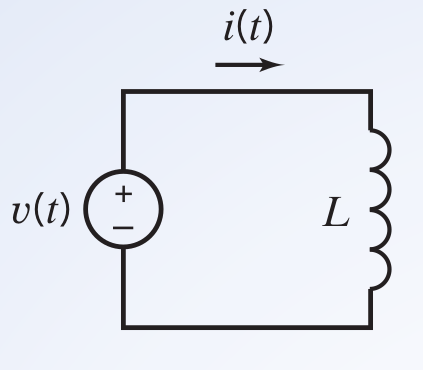
\includegraphics[height=.7\textwidth]{figura9.png}	
		    \end{center}
		\end{column}
		
		  \begin{column}{.3\textwidth}  %%<--- here
		    \begin{center}
    	  		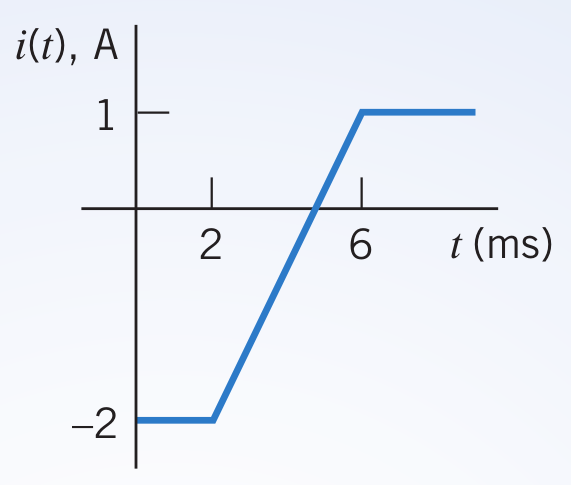
\includegraphics[height=.7\textwidth]{figura10.png}	
		    \end{center}
		\end{column}
	
	
	
	\end{columns}\\
	

	
	
	 \begin{columns}
		\begin{column}{1\textwidth}
	\newline	\scalebox{0.8}{Answer: $L=40mH.$}
		\end{column}
	  \end{columns}\\
	
	
\end{tabular}
\end{frame}





% ----------------- NOVO SLIDE --------------------------------
\begin{frame}[fragile]
\frametitle{Capacitor Current and Voltage}
\begin{tabular}{r}

	    \begin{columns}
		\begin{column}{1\textwidth}
		\textbf{EXAMPLE 7.2-5} - The input to the circuit shown in Figure below is the current 
		\end{column}
	  \end{columns}\\
	    \begin{columns}
	    
	    	\begin{column}{.3\textwidth}  %%<--- here
		    \begin{center}
    	  		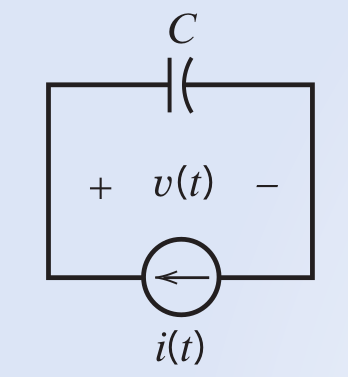
\includegraphics[height=.7\textwidth]{figura11.png}	
		    \end{center}
		\end{column}
	    
		\begin{column}{.5\textwidth}
		  \begin{center} $i(t)=3.75e^{-1.2t} \ A \ (t>0)$.\end{center}
		\end{column}
	%  \end{columns}\\
	%	\begin{columns}

	\end{columns}\\
	
	    \begin{columns}
		\begin{column}{1\textwidth}
		\newline The output is the capacitor voltage  $v(t)=4-1.25e^{-1.2t} \ V \ (t>0)$. Find the value of the capacitance $C$. \newline \\
		\end{column} 
	  \end{columns}\\

	
\end{tabular}

	  
\scalebox{0.8}{Answer: $C=2.5  F.$}  	   

\end{frame}





% ----------------- NOVO SLIDE --------------------------------
\begin{frame}[fragile]
\frametitle{Inductor Current and Voltage}
\begin{tabular}{r}

	    \begin{columns}
		\begin{column}{1\textwidth}
		\textbf{EXAMPLE 7.5-3} - The input to the circuit shown in Figure below is the voltage 
		\end{column}
	  \end{columns}\\
	    \begin{columns}
	    
	    	\begin{column}{.3\textwidth}  %%<--- here
		    \begin{center}
    	  		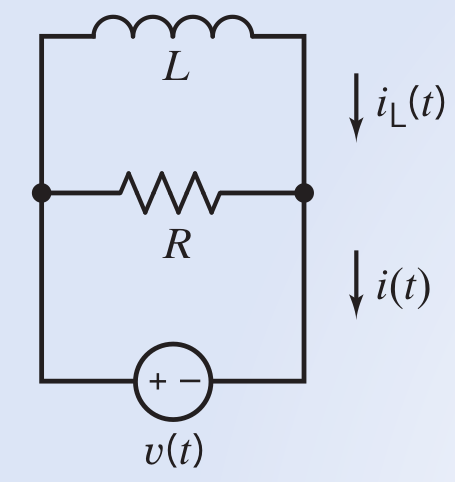
\includegraphics[height=.8\textwidth]{figura12.png}	
		    \end{center}
		\end{column}
	    
		\begin{column}{.5\textwidth}
		  \begin{center} $v(t)=4e^{-20t} \ V \ (t>0)$.\end{center}
		\end{column}
	%  \end{columns}\\
	%	\begin{columns}

	\end{columns}\\
	
	    \begin{columns}
		\begin{column}{1\textwidth}
		\newline The output is the current $i(t)=-1.2e^{-20t}-1.5 \ A \ (t>0)$.The initial inductor current is $i_{L}(0)=-3.5 \ A$. Determine the values of the inductance
$L$ and resistance $R$. \newline\\
		\end{column} 
	  \end{columns}\\

	
\end{tabular}

	  
	  
\scalebox{0.8}{Answer: $L=0.1H \ R=5 \Omega$.} 	   

\end{frame}


% ----------------- NOVA SECÇÂO -----------------------------
\section{Energy Storage in a Capacitor (7.3) and Inductor (7.6)}
% ----------------- NOVO SLIDE --------------------------------

\begin{frame}[fragile]
\frametitle{Energy Storage in a Capacitor}
	
	
	\begin{tabular}{r}

	\begin{columns}
		\begin{column}{1\textwidth}
		The forces acting on the charges stored in a capacitor are said to result from an \textbf{electric field}. 
		The energy stored in a capacitor is 
		\end{column}
	  \end{columns}\\

	  \begin{columns}
		  \begin{column}{.5\textwidth}  %%<--- here
		%
\large 				\begin{flushleft} 
					$w_{C}(t)=\int_{-\infty}^{t} v(\tau)i(\tau) d\tau \ J$ 
					\end{flushleft}
\scriptsize				\begin{flushleft} 
					$i(\tau)=C \frac{dv(\tau)}{d \tau}$
					\end{flushleft}			
					\begin{flushleft} 
					$w_{C}(t)=\int_{-\infty}^{t} v(\tau)C \frac{dv(\tau)}{d \tau} d\tau$
					\end{flushleft}
					\begin{flushleft} 
					$w_{C}(t)=C\int_{v(-\infty)}^{v(t)} v(\tau) dv(\tau) $
					\end{flushleft}

		\end{column}
		
		  \begin{column}{.4\textwidth}  %%<--- here
\scriptsize		   		\begin{flushleft} 
					$w_{C}(t)=C\frac{1}{2}v^2(t) \Big|_{v(-\infty)=0}^{v(t)} $
					\end{flushleft}
					
\large 				\begin{flushleft} 			 
					$w_{C}(t)=\frac{1}{2}Cv^2(t) \ J$
					\end{flushleft}
		   			
\scriptsize		   		\begin{flushleft} 
					$v(t)=\frac{q(t)}{C}$  
					\end{flushleft}
					
\large 				\begin{flushleft}
					 $w_{C}(t)=\frac{1}{2C}q^2(t) \ J$
					\end{flushleft}
 

					
		\end{column}
	

	
	\end{columns}\\
		\begin{columns}
		\begin{column}{1\textwidth}
\newline	\newline	The capacitor is a storage element that stores but does not dissipate energy.	
		\end{column}
	  \end{columns}\\
	

	
\end{tabular}
	
	
\end{frame}
% ----------------- NOVO SLIDE --------------------------------

\begin{frame}[fragile]
\frametitle{Energy Storage in a Inductor}
	
	
	\begin{tabular}{r}

	\begin{columns}
		\begin{column}{1\textwidth}
		The energy stored in the inductor is stored in its \textbf{magnetic field}. The energy stored in the inductor during
the interval $-\infty$ to $t$ is given by 
		\end{column}
	  \end{columns}\\

	  \begin{columns}
		  \begin{column}{.5\textwidth}  %%<--- here
		%
\large 				\begin{flushleft} 
					$w_{L}(t)=\int_{-\infty}^{t} v(\tau)i(\tau) d\tau \ J$ 
					\end{flushleft}
\scriptsize				\begin{flushleft} 
					$v(\tau)=L \frac{di(\tau)}{d \tau}$
					\end{flushleft}			
					\begin{flushleft} 
					$w_{L}(t)=\int_{-\infty}^{t} L \frac{di(\tau)}{d \tau} i(\tau) d\tau$
					\end{flushleft}
					\begin{flushleft} 
					$w_{L}(t)=L\int_{i(-\infty)}^{i(t)} i(\tau) di(\tau) $
					\end{flushleft}

		\end{column}
		
		  \begin{column}{.4\textwidth}  %%<--- here
\scriptsize		   		\begin{flushleft} 
					$w_{L}(t)=L\frac{1}{2}i^2(t) \Big|_{i(-\infty)=0}^{i(t)} $
					\end{flushleft}
					
\large 				\begin{flushleft} 			 
					$w_{L}(t)=\frac{1}{2}Li^2(t) \ J$
					\end{flushleft}
		   			
\scriptsize		   		\begin{flushleft} 
					$i(t)=\frac{\phi(t)}{L}$  
					\end{flushleft}
					
\large 				\begin{flushleft}
					 $w_{L}(t)=\frac{1}{2L}\phi^2(t) \ J$
					\end{flushleft}
 

					
		\end{column}
	

	
	\end{columns}\\
		\begin{columns}
		\begin{column}{1\textwidth}
\newline	\newline	The inductor is a storage element that stores but does not dissipate energy.	
		\end{column}
	  \end{columns}\\
	

	
\end{tabular}
	
	
\end{frame}

% ----------------- NOVO SLIDE --------------------------------
\begin{frame}[fragile]
\frametitle{Capacitor Current, Voltage, Power and Energy}
\begin{tabular}{r}
	    \begin{columns}
		\begin{column}{1\textwidth}
		\textbf{EXAMPLE 7.3-2} - The voltage across a 5mF capacitor varies as shown in
Figure below. Determine and plot the capacitor current, power, and energy. \\
		\end{column}
	  \end{columns}\\
		\begin{columns}
		  \begin{column}{.7\textwidth}  %%<--- here
		    \begin{center}
    	  		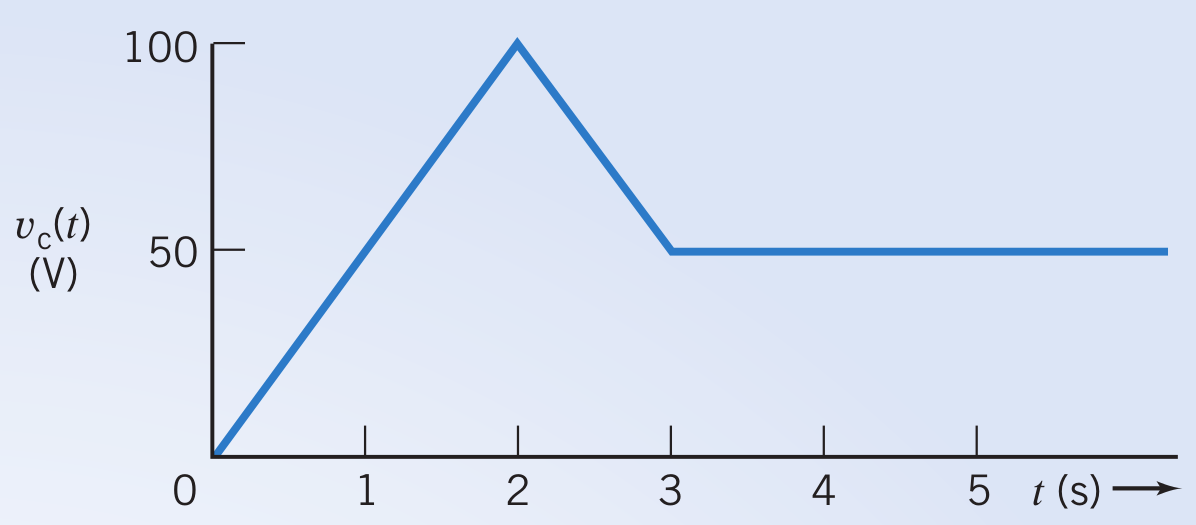
\includegraphics[height=.4\textwidth]{figure13.png}	
		    \end{center}
		\end{column}
		
	 
	
	
	
	\end{columns}
	

	
\end{tabular}
\end{frame}

% ----------------- NOVO SLIDE --------------------------------
\begin{frame}[fragile]
\frametitle{Inductor Current, Voltage, Power and Energy}
\begin{tabular}{r}
	    \begin{columns}
		\begin{column}{1\textwidth}
		\textbf{EXAMPLE 7.6-2} - Find the power and energy for an inductor of 0.1H
when the current and voltage are as shown in Figures below. \newline \\
		\end{column}
	  \end{columns}\\
		\begin{columns}
		  \begin{column}{1.2\textwidth}  %%<--- here
		    \begin{center}
    	  		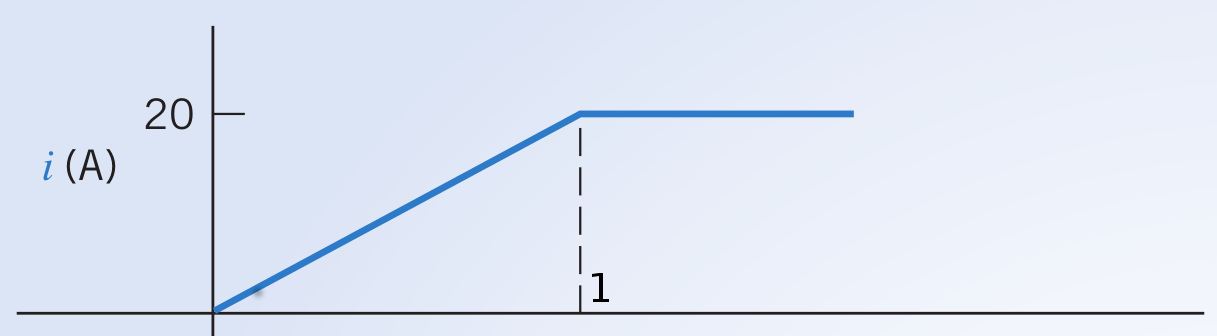
\includegraphics[width=7cm,height=3.5cm]{figure14.png}	{}
    	  		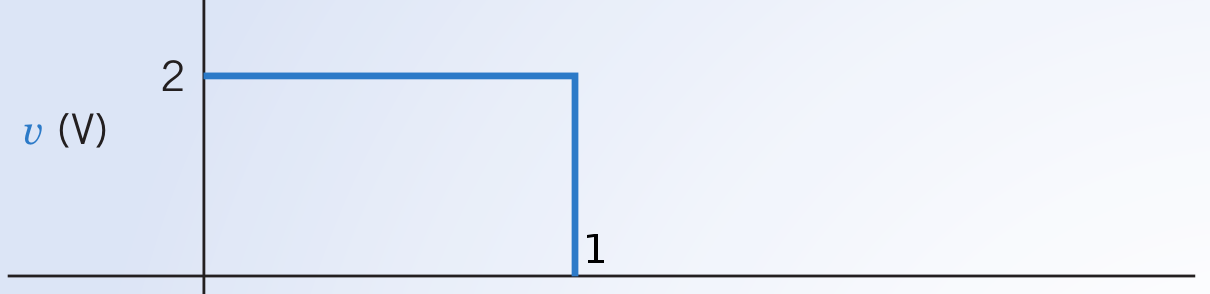
\includegraphics[width=7cm,height=3.5cm]{figure15.png}
		    \end{center}
		\end{column}
		
	 
	
	
	
	\end{columns}
	

	
\end{tabular}
\end{frame}


% ----------------- NOVA SECÇÂO -----------------------------
\section{Series and Parallel Capacitor (7.4) and Inductor (7.7)}
% ----------------- NOVO SLIDE --------------------------------
\begin{frame}[fragile]
\frametitle{Parallel Capacitor}
\begin{tabular}{r}
	    \begin{columns}
		\begin{column}{1\textwidth}
		First, let us consider the parallel connection of N capacitors as shown in
Figure below. \\
		\end{column}
	  \end{columns}\\
		\begin{columns}
		  \begin{column}{.5\textwidth}  %%<--- here
		    \begin{center}
    	  		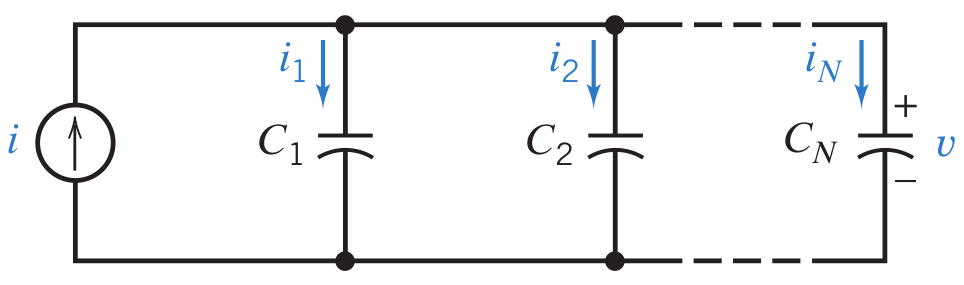
\includegraphics[width=6cm,height=2.0cm]{figure16.png}\\
    	\tiny  		Parallel connection of N capacitors\\
    	  		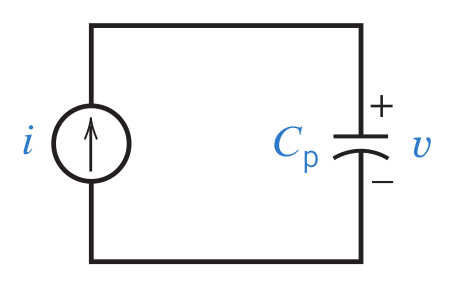
\includegraphics[width=3cm,height=2.0cm]{figure17.png}\\
    	  		Equivalent circuit for N parallel capacitors.
		    \end{center}
		\end{column}
		
	 		  \begin{column}{.5\textwidth}  %%<--- here

   \scriptsize   	  		\begin{flushleft} 
    	  		Using KCL, we have\\
  	  		 $i=i_1+i_2+i_3+...+i_N$ \newline
    	  	\newline	 Because\\ 
    	  		  $i_n=C_n \frac{dv}{dt}$ \newline
    	  	\newline	  We obtain\\
    	  		 $i=C_1 \frac{dv}{dt}+C_2 \frac{dv}{dt}+C_3 \frac{dv}{dt}+...+C_N \frac{dv}{dt}$ 
    	  		 $i=(C_1+C_2+C_3+...+C_N) \frac{dv}{dt} = C_p\frac{dv}{dt}$ \newline
  \normalsize  	  	\newline	 $C_p=\sum_{n=1}^{N} C_n$ 
    	  		\end{flushleft}

		\end{column}
	
	
	
	\end{columns}
	

	
\end{tabular}	
\end{frame}
% ----------------- NOVO SLIDE --------------------------------
\begin{frame}[fragile]
\frametitle{Series Capacitor}
\begin{tabular}{r}
	    \begin{columns}
		\begin{column}{1\textwidth}
		Now let us determine the equivalent capacitance $C_s$ of a set of N
series-connected capacitances, as shown in Figure below. \\
		\end{column}
	  \end{columns}\\
		\begin{columns}
		  \begin{column}{.5\textwidth}  %%<--- here
		    \begin{center}
    	  		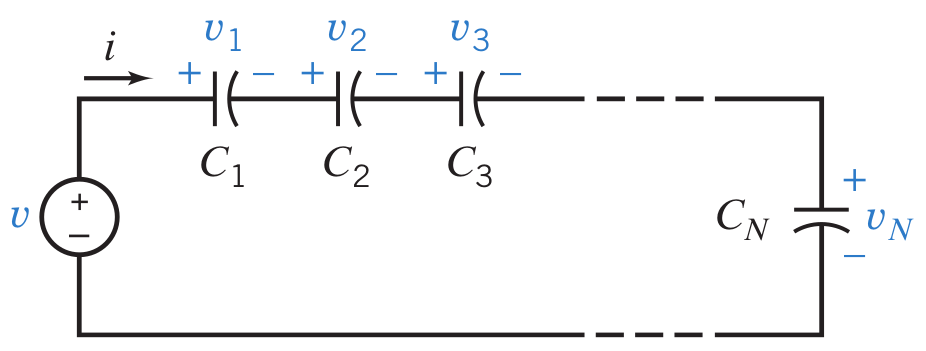
\includegraphics[width=6cm,height=2.0cm]{figure18.png}\\
    	\tiny  		Serie connection of N capacitors\\
    	  		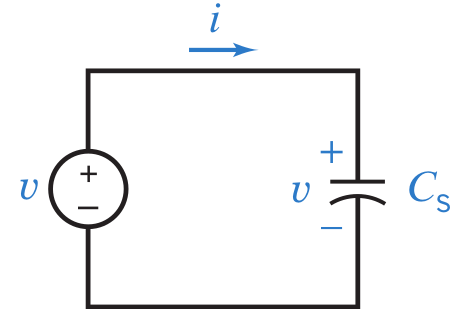
\includegraphics[width=3cm,height=2.0cm]{figure19.png}\\
    	  		Equivalent circuit for N Serie capacitors.
		    \end{center}
		\end{column}
		
	 		  \begin{column}{.5\textwidth}  %%<--- here

   \scriptsize   	  		\begin{flushleft} 
    	  		Using KVL, we have\\
  	  		 $v=v_1+v_2+v_3+...+v_N$ \newline
    	  	\newline	 Because\\ 
    	  		  $v_n(t)=\frac{1}{C_n}\int_{t_{0}}^{t} i d\tau+v_n(t_{0})$ \newline
    	  	\newline	  We obtain\\
    	  		 $v=\frac{1}{C_1}\int_{t_{0}}^{t} i d\tau+v_1(t_{0})+...+\frac{1}{C_N}\int_{t_{0}}^{t} i d\tau+v_N(t_{0})$ 
    	  		 $v=(\frac{1}{C_1}+\frac{1}{C_2}+...+\frac{1}{C_N})\int_{t_{0}}^{t} i d\tau+\sum_{n=1}^{N} v_N(t_{0})$  \newline
  \normalsize  	  	\newline	 $\frac{1}{C_s}=\sum_{n=1}^{N} \frac{1}{C_n}$ 
    	  		\end{flushleft}

		\end{column}
	
	
	
	\end{columns}
	

	
\end{tabular}	
\end{frame}

% ----------------- NOVO SLIDE --------------------------------
\begin{frame}[fragile]
\frametitle{Series Inductor}
\begin{tabular}{r}
	    \begin{columns}
		\begin{column}{1\textwidth}
		Consider a series connection of N inductors as shown in Figure below. \\
		\end{column}
	  \end{columns}\\
		\begin{columns}
		  \begin{column}{.5\textwidth}  %%<--- here
		    \begin{center}
    	  		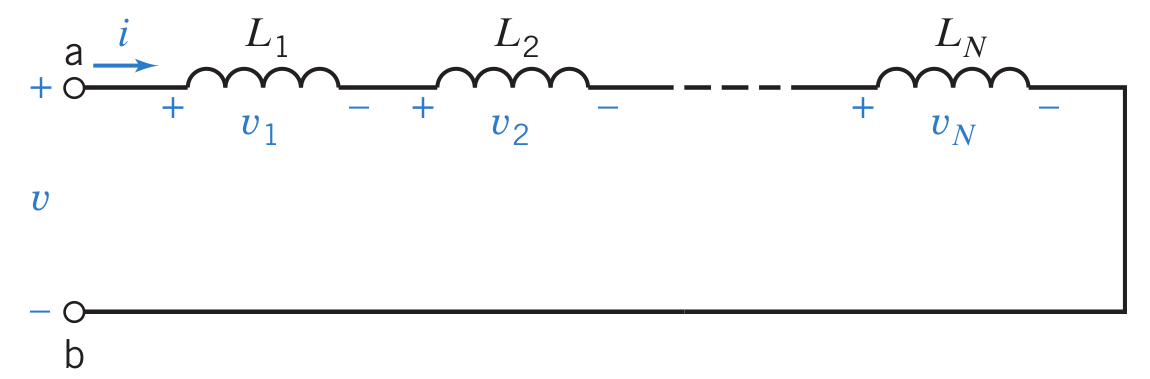
\includegraphics[width=6cm,height=2.0cm]{figure20.png}\\
    	\tiny  		Serie connection of N inductors\\
    	  		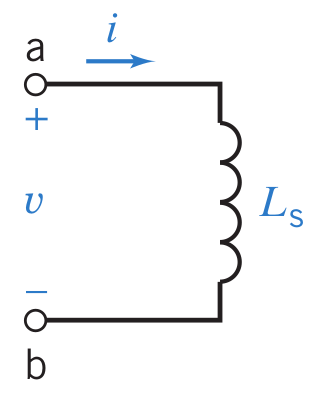
\includegraphics[width=3cm,height=2.0cm]{figure21.png}\\
    	  		Equivalent circuit for N Serie inductors.
		    \end{center}
		\end{column}
		
		
	 		  \begin{column}{.5\textwidth}  %%<--- here

   \scriptsize   	  		\begin{flushleft} 
    	  		Using KVL, we have\\
  	  		 $v=v_1+v_2+v_3+...+v_N$ \newline
    	  	\newline	 Because\\ 
    	  		  $v_n=L_n \frac{di}{dt}$ \newline
    	  	\newline	  We obtain\\
    	  		 $v=L_1 \frac{di}{dt}+L_2 \frac{di}{dt}+L_3 \frac{di}{dt}+...+L_N \frac{di}{dt}$ 
    	  		 $v=(L_1+L_2+L_3+...+L_N) \frac{di}{dt} = L_s\frac{di}{dt}$ \newline
  \normalsize  	  	\newline	 $L_s=\sum_{n=1}^{N} L_n$ 
    	  		\end{flushleft}

		\end{column}
	
	
	
	\end{columns}
	

	
\end{tabular}	
\end{frame}

% ----------------- NOVO SLIDE --------------------------------

\begin{frame}[fragile]
\frametitle{Parallel Inductor}
\begin{tabular}{r}
	    \begin{columns}
		\begin{column}{1\textwidth}
		Now, consider the set of N inductors in parallel, as shown in Figure below. \\
		\end{column}
	  \end{columns}\\
		\begin{columns}
		  \begin{column}{.5\textwidth}  %%<--- here
		    \begin{center}
    	  		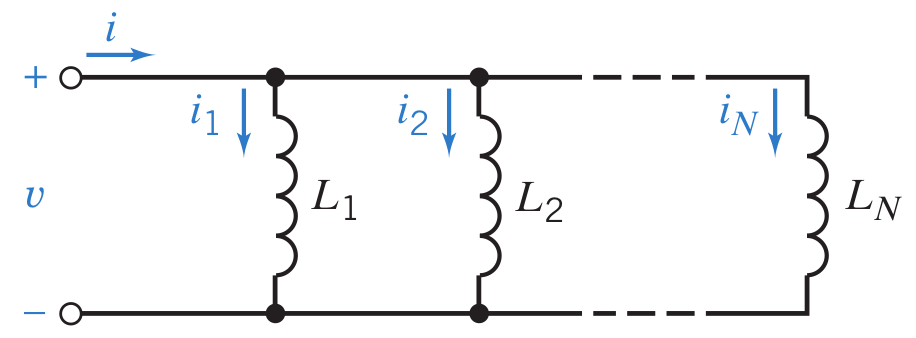
\includegraphics[width=6cm,height=2.0cm]{figure22.png}\\
    	\tiny  		Parallel connection of N inductors\\
    	  		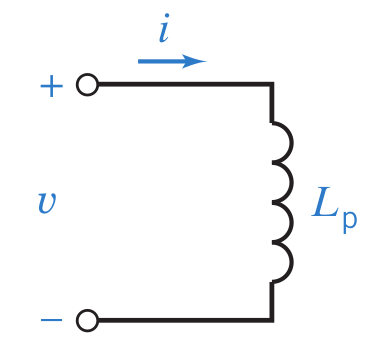
\includegraphics[width=3cm,height=2.0cm]{figure23.png}\\
    	  		Equivalent circuit for N parallel inductors.
		    \end{center}
		\end{column}
		
	 		  \begin{column}{.5\textwidth}  %%<--- here

   \scriptsize   	  		\begin{flushleft} 
    	  		Using KCL, we have\\
  	  		 $i=i_1+i_2+i_3+...+i_N$ \newline
    	  	\newline	 Because\\ 
    	  		  $i_n(t)=\frac{1}{L_n}\int_{t_{0}}^{t} v d\tau+i_n(t_{0})$ \newline
    	  	\newline	  We obtain\\
    	  		 $i=\frac{1}{L_1}\int_{t_{0}}^{t} v d\tau+i_1(t_{0})+...+\frac{1}{L_N}\int_{t_{0}}^{t} v d\tau+i_N(t_{0})$ 
    	  		 $i=(\frac{1}{L_1}+\frac{1}{L_2}+...+\frac{1}{L_N})\int_{t_{0}}^{t} v d\tau+\sum_{n=1}^{N} i_n(t_{0})$  \newline
  \normalsize  	  	\newline	 $\frac{1}{L_p}=\sum_{n=1}^{N} \frac{1}{L_n}$ 
    	  		\end{flushleft}

		\end{column}
	
	
	
	\end{columns}
	

	
\end{tabular}	
\end{frame}



% ----------------- NOVO SLIDE --------------------------------
\begin{frame}[fragile]
\frametitle{Series and Parallel Capacitor}
\begin{tabular}{r}
	    \begin{columns}
		\begin{column}{1\textwidth}
		\textbf{EXAMPLE 7.4-1} - Find the equivalent capacitance for the circuit of Figure below when
$C_1=C_2=C_3=2 mF, \ v_1(0)=10V, and \ v_2(0)=v_3(0)=20 V$. \newline \\
		\end{column}
	  \end{columns}\\
		\begin{columns}
		  \begin{column}{1.2\textwidth}  %%<--- here
		    \begin{center}
    	  		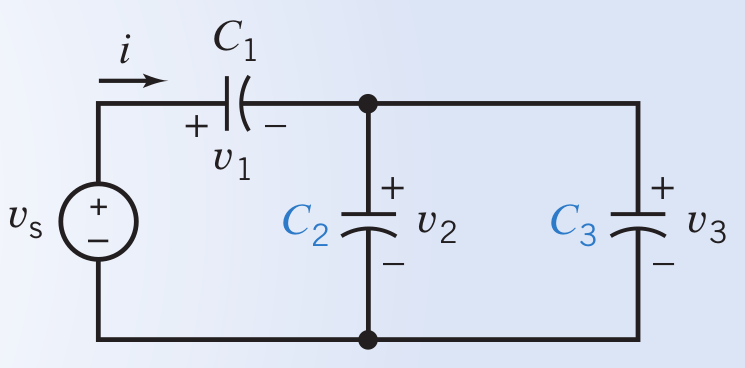
\includegraphics[width=7cm,height=3.5cm]{figure24.png}
		    \end{center}
		\end{column}
		
	 
	
	
	
	\end{columns}\\
	  \begin{columns}
		\begin{column}{1\textwidth}
\scalebox{0.8}{Answer: $C_{eq}=\frac{8}{6}  mF \ and \ v_s(0)=30V.$}  
		\end{column}
	  \end{columns}\\		

	
\end{tabular}
\end{frame}

% ----------------- NOVO SLIDE --------------------------------
\begin{frame}[fragile]
\frametitle{Series and Parallel inductor}
\begin{tabular}{r}
	    \begin{columns}
		\begin{column}{1\textwidth}
		\textbf{EXAMPLE 7.7-1} - Find the equivalent inductance for the circuit of Figure below. All the
inductor currents are zero at $t_0$. \newline \\
		\end{column}
	  \end{columns}\\
		\begin{columns}
		  \begin{column}{1.2\textwidth}  %%<--- here
		    \begin{center}
    	  		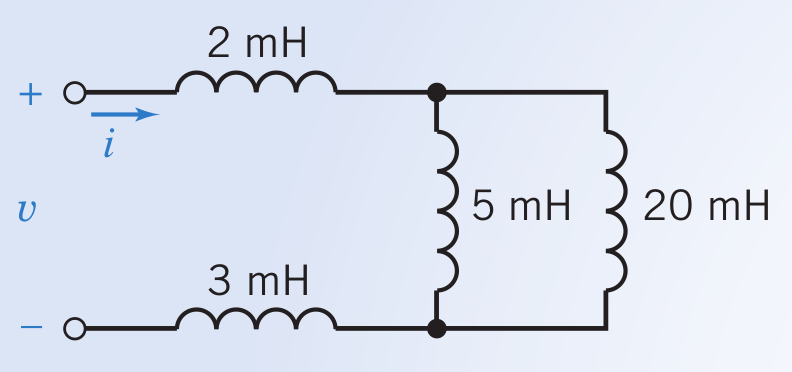
\includegraphics[width=7cm,height=3.5cm]{figure25.png}
		    \end{center}
		\end{column}
		
	 
	
	
	
	\end{columns}\\
	
	
	  \begin{columns}
		\begin{column}{1\textwidth}
\scalebox{0.8}{Answer: $L_{eq}=9mH.$}  
		\end{column}
	  \end{columns}\\

	
	
\end{tabular}
\end{frame}





% ----------------- NOVA SECÇÂO -----------------------------
\section{Initial Conditions of Switched Circuits (7.8)}
% ----------------- NOVO SLIDE --------------------------------
\begin{frame}[fragile]
\frametitle{Initial Conditions of Switched Circuits}

\begin{tabular}{r}
	    \begin{columns}
	     \begin{column}{.5\textwidth}  %%<--- here
	     Our plan to analyze switched circuits has two steps: \newline
   \scriptsize 						\begin{itemize}
						\item[$\clubsuit$]{Analyze the dc circuit that exists before time $t_0$ to determine the capacitor voltages and inductor
currents. In doing this analysis, we will take advantage of the fact that capacitors behave as open circuits, $i(t)=C\frac{d}{dt}v(t)$,
and inductors behave as short circuits, $v(t)=L\frac{d}{dt}i(t)$, when they are in dc circuits;}
						\item[$\clubsuit$]{Recognize that capacitor voltages and inductor currents cannot change instantaneously, so
the capacitor voltages and inductor currents at time $t^+_0$ have the same values that they had at time $t^-_0$.}
\end{itemize}
\end{column}
		
					

		  \begin{column}{.5\textwidth}  %%<--- here
		    \begin{center}
  \scriptsize \flushleft \textbf{EXAMPLE 7.8-1} - Consider the circuit Figure below. Prior to $t=0$, the switch has been closed for a long time. Determine the values of
the capacitor voltage and inductor current immediately after the switch opens at time $t=0$. \newline \\				  
    	  		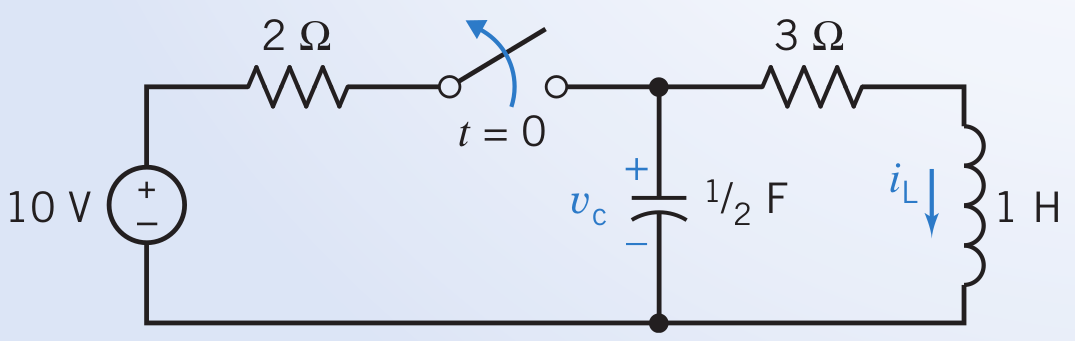
\includegraphics[width=6cm,height=1.7cm]{figure26.png}\\ 

    		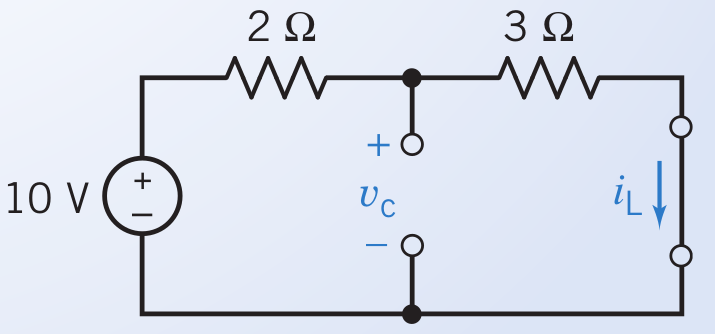
\includegraphics[width=3cm,height=1.7cm]{figure27.png}\\
	\scalebox{0.8}{Answer: $v_C(0^-)=v_C(0^+)=6V \ and \ i_L(0^-)=i_L(0^+)=2A$}
		    \end{center}

	\end{column}
		
	 
	
	
	
	\end{columns}
	

	
\end{tabular}
\end{frame}
	
% ----------------- NOVO SLIDE --------------------------------
\begin{frame}[fragile]
\frametitle{Initial Conditions of Switched Circuits}
\begin{tabular}{r}
	    \begin{columns}
		\begin{column}{1\textwidth}
		\textbf{EXAMPLE 7.8-2} - Find $i_L(0^+)$, $v_C(0^+)$, $\frac{dv_C(0^+)}{dt}$, and $\frac{di_L(0^+)}{dt}$ for the circuit of Figure below.\\
		\end{column}
	  \end{columns}\\
		\begin{columns}
		  \begin{column}{1\textwidth}  %%<--- here
		    \begin{center}
    	  		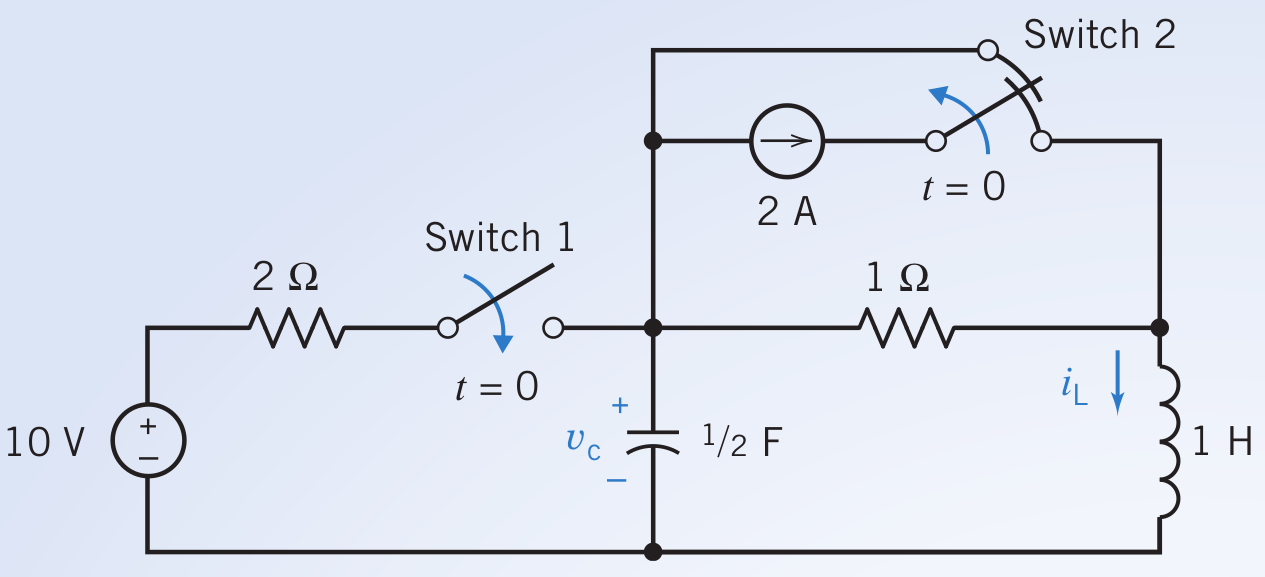
\includegraphics[width=7cm,height=3.5cm]{figure38.png}
		    \end{center}
		\end{column}
		
	 
	
	
	
	\end{columns}\\
	
	
	  \begin{columns}
		\begin{column}{1\textwidth}
\newline \scalebox{0.8}{Answer: $i_L(0^+)=0A$, $v_C(0^+)=-2V$, $\frac{dv_C(0^+)}{dt}=12V/s$, and $\frac{di_L(0^+)}{dt}=-2A/s$.}  
		\end{column}
	  \end{columns}\\

	
	
\end{tabular}
\end{frame}


% ----------------- NOVO SLIDE --------------------------------
\begin{frame}[fragile]
\frametitle{Initial Conditions of Switched Circuits}
\begin{tabular}{r}
	    \begin{columns}
		\begin{column}{1\textwidth}
\small		\textbf{PROBLEM 7.8-2} - The switch in Figure below has been open for a long time before closing at time $t=0$. Find $v_C(0^+)$ and $i_L(0^+)$, the
values of the capacitor voltage and inductor current immediately after the switch closes. Let $v_C(\infty)$ and $i_L(\infty)$ denote the values of the capacitor voltage and inductor current after the switch has been closed for a long time. 
Find $v_C(\infty)$ and $i_L(\infty)$.
		\end{column}
	  \end{columns}\\
		\begin{columns}
		  \begin{column}{1\textwidth}  %%<--- here
	%	    \begin{center}
    	 \center 		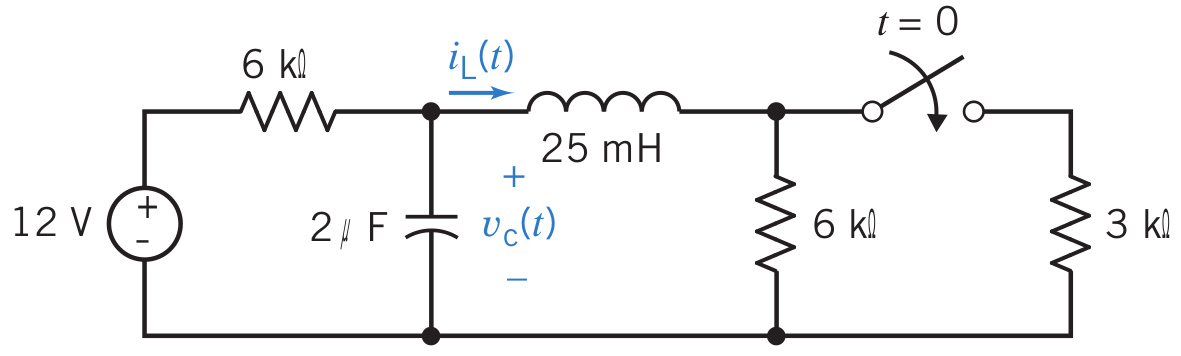
\includegraphics[width=7cm,height=2.5cm]{figure39.png}
	%	    \end{center}
		\end{column}	
	\end{columns}\\
	
	
	  \begin{columns}
		\begin{column}{1\textwidth}
\newline \scalebox{0.8}{Answer:$v_C(0^+)=6V$, $i_L(0^+)=1mA$, $v_C(\infty)=3V$, and $i_L(\infty)=1.5mA$.}  
		\end{column}
	  \end{columns}\\

	
	
\end{tabular}
\end{frame}
% ----------------- NOVO SLIDE --------------------------------
\begin{frame}[fragile]
\frametitle{Initial Conditions of Switched Circuits}
\begin{tabular}{r}
	    \begin{columns}
		\begin{column}{1\textwidth}
\small		\textbf{PROBLEM 7.8-11} -The circuit shown in Figure below has reached
steady state before the switch opens at time $t=0$. Determine the
values of $i_L(t)$, $v_C(t)$, and $v_R(t)$ immediately before the switch opens
and the value of $v_R(t)$ immediately after the switch opens.
		\end{column}
	  \end{columns}\\
		\begin{columns}
		  \begin{column}{1\textwidth}  %%<--- here
	%	    \begin{center}
    	 \center 		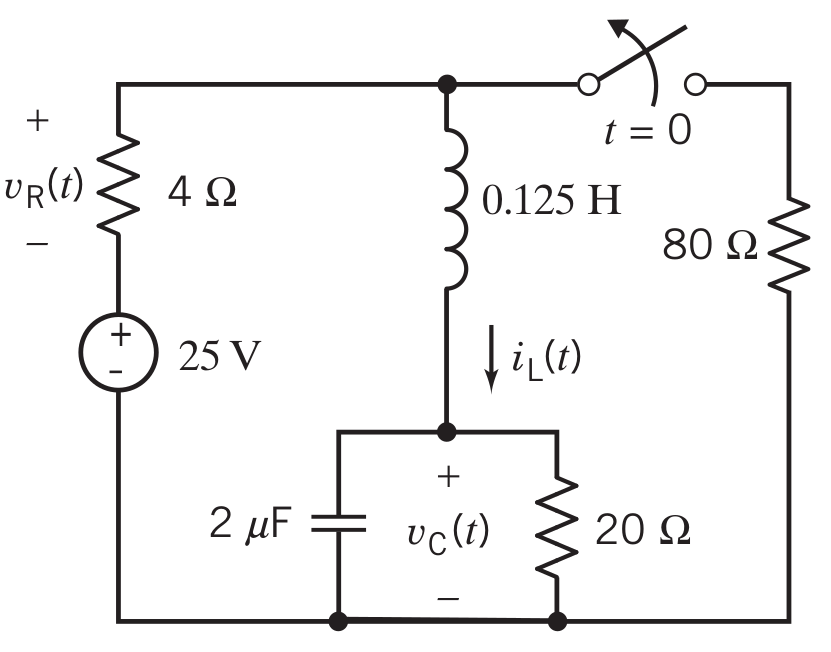
\includegraphics[width=7cm,height=3.5cm]{figure40.png}
	%	    \end{center}
		\end{column}	
	\end{columns}\\
	
	
	  \begin{columns}
		\begin{column}{1\textwidth}
\newline \scalebox{0.8}{Answer: $i_L(0^-)=1A$, $v_C(0^-)=20V$, $v_R(0^-)=-5V$, and $v_R(0^+)=-4V$.}  
		\end{column}
	  \end{columns}\\

	
	
\end{tabular}
\end{frame}




% ----------------- NOVA SECÇÂO -----------------------------
\section{Operational Amplifier Circuits and Linear Differential Equations (7.9)}
% ----------------- NOVO SLIDE --------------------------------
\begin{frame}[fragile]
\frametitle{Operational Amplifier Circuits and Linear Differential Equations}

\begin{tabular}{r}
	    \begin{columns}
	      \begin{column}{1\textwidth}  %%<--- here
	This section describes a procedure for designing operational amplifier circuits that implement linear differential equations such as
	\\ \center $2\frac{d^3}{dt^3}y(t)+5\frac{d^2}{dt^2}y(t)+4\frac{d}{dt}y(t)+3y(t)=6x(t)$
	     \end{column}

	  \end{columns}
	  \end{tabular}
\begin{tabular}{c}
		\begin{columns}
		  \begin{column}{.5\textwidth}  %%<--- here
		    \begin{center}
    	  		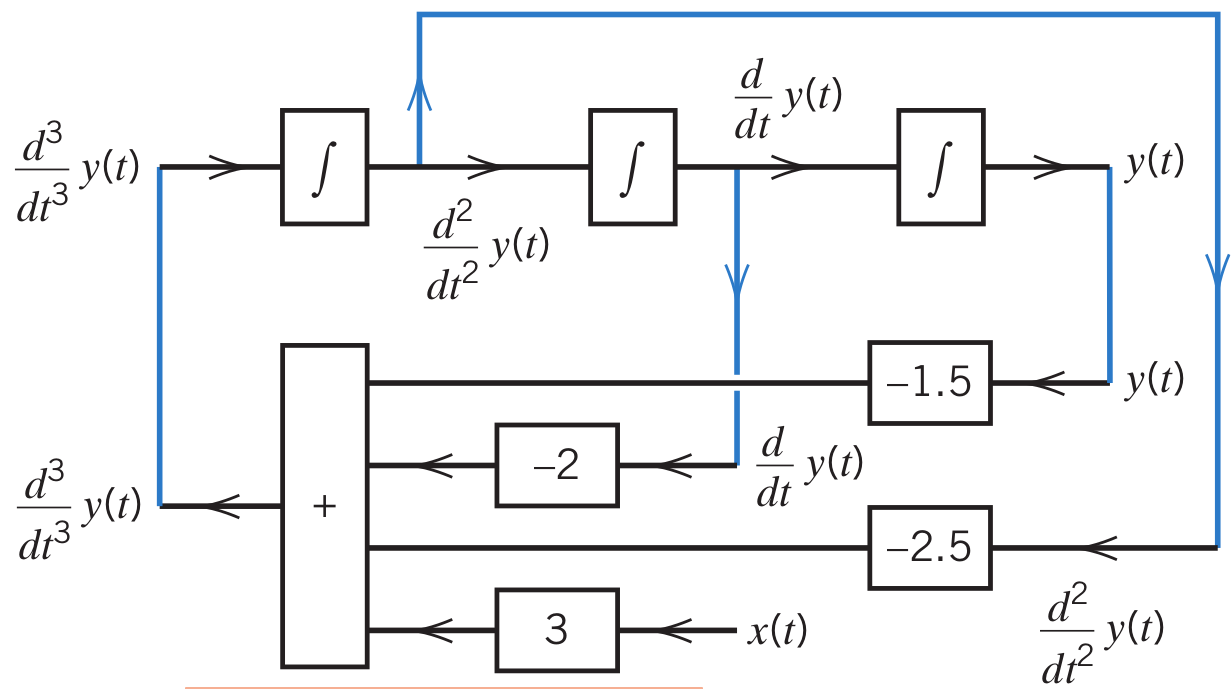
\includegraphics[height=.45\textwidth]{figure28.png}	
		    \end{center}
		\end{column}
		\begin{column}{.25\textwidth}  %%<--- here
		    \begin{center}
    	  		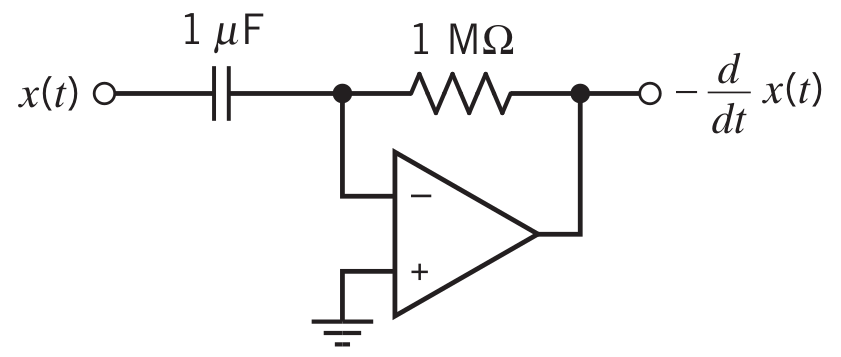
\includegraphics[width=2.8cm,height=2cm]{figure30.png}\\
    	  		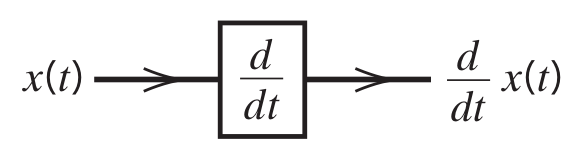
\includegraphics[width=2.8cm,height=1.2cm]{figure33.png}\\
    	  		
		    \end{center}
		\end{column}
		\begin{column}{.25\textwidth}  %%<--- here
		    \begin{center}
    	  		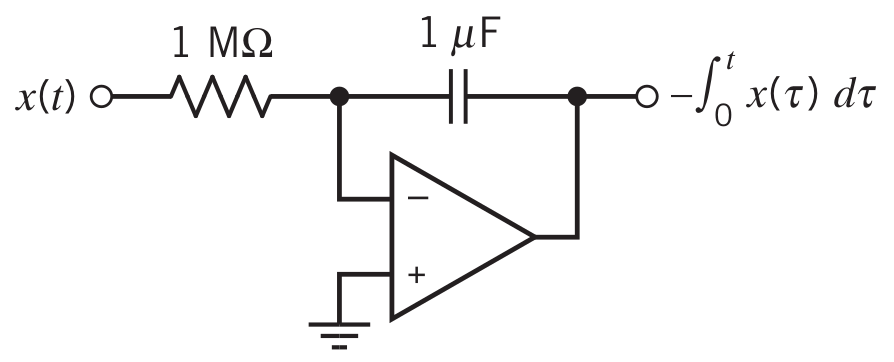
\includegraphics[width=2.8cm,height=2cm]{figure32.png}\\
    	  		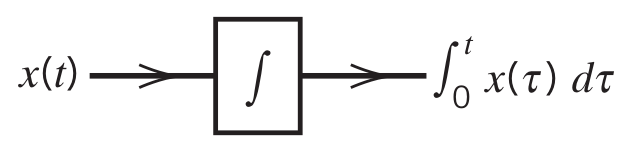
\includegraphics[width=2.8cm,height=1.2cm]{figure31.png}\\
    	  		
		    \end{center}
		\end{column}
	\end{columns}\\
			\begin{columns}
		  \begin{column}{.5\textwidth}  %%<--- here
		    \begin{center}
    	  \tiny		A block diagram that represents	
		    \end{center}
		\end{column}
			  \begin{column}{.25\textwidth}  %%<--- here
		    \begin{center}
    	  \tiny		Differentiation	
		    \end{center}
		\end{column}
		  \begin{column}{.25\textwidth}  %%<--- here
		    \begin{center}
    	  \tiny		Integration	
		    \end{center}
		\end{column}
	\end{columns}

	
\end{tabular}
\end{frame}
% ----------------- NOVO SLIDE --------------------------------
\begin{frame}[fragile]
\frametitle{Operational Amplifier Circuits and Linear Differential Equations}

\begin{tabular}{r}
	    \begin{columns}
	    		  \begin{column}{1\textwidth}  %%<--- here
	This section describes a procedure for designing operational amplifier circuits that implement linear differential equations such as
	\\ \center $2\frac{d^3}{dt^3}y(t)+5\frac{d^2}{dt^2}y(t)+4\frac{d}{dt}y(t)+3y(t)=6x(t)$
		      		\end{column}

	  \end{columns}\\
		\begin{columns}
		  \begin{column}{.5\textwidth}  %%<--- here
		    \begin{center}
    	  		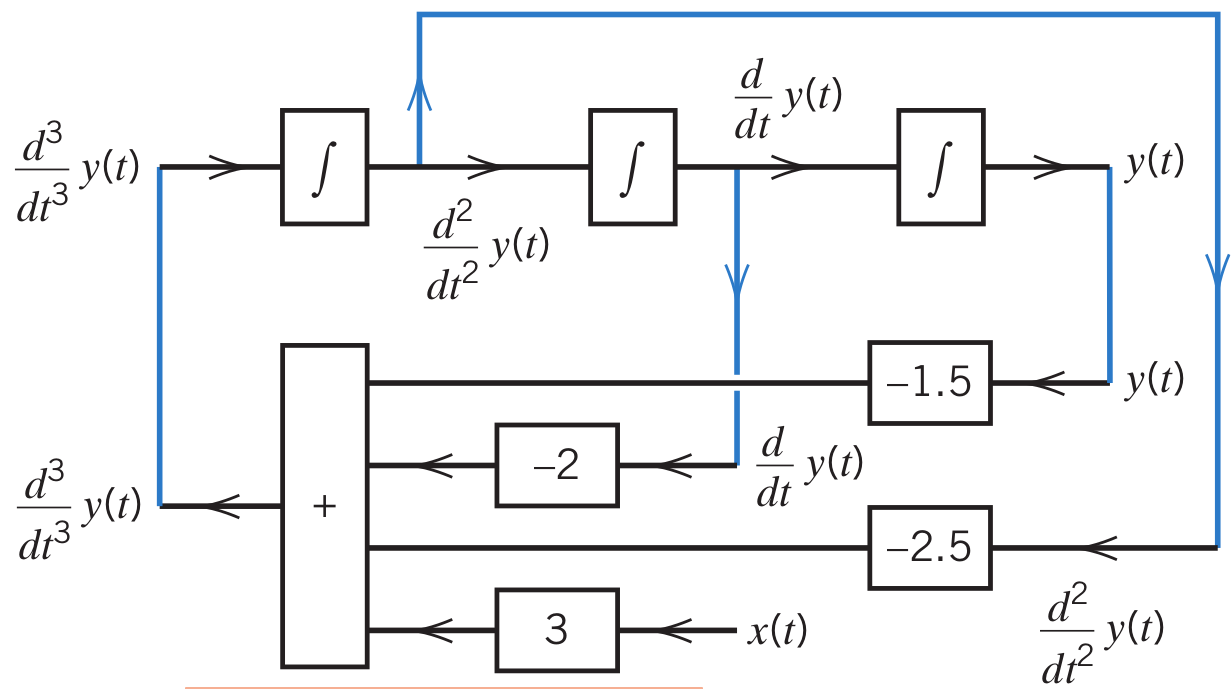
\includegraphics[height=.45\textwidth]{figure28.png}	
		    \end{center}
		\end{column}
			  \begin{column}{.5\textwidth}  %%<--- here
		    \begin{center}
    	  		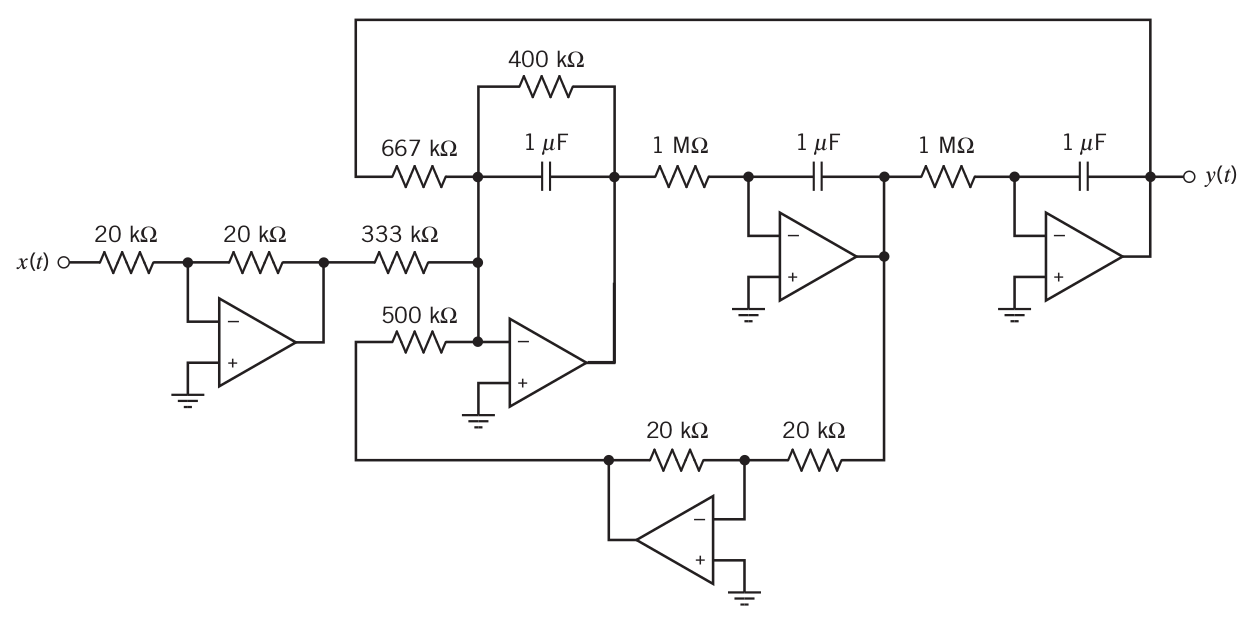
\includegraphics[height=.45\textwidth]{figure29.png}	
		    \end{center}
		\end{column}
	\end{columns}\\
			\begin{columns}
		  \begin{column}{.5\textwidth}  %%<--- here
		    \begin{center}
    	  \tiny		A block diagram that represents	
		    \end{center}
		\end{column}
			  \begin{column}{.5\textwidth}  %%<--- here
		    \begin{center}
    	  \tiny		An operational amplifier circuit that implements	
		    \end{center}
		\end{column}
	\end{columns}

	
\end{tabular}
\end{frame}
	
% ----------------- NOVA SECÇÂO -----------------------------
\section{Using MATLAB to Plot Capacitor or Inductor Voltage and Current (7.10)}
% ----------------- NOVO SLIDE --------------------------------
\begin{frame}[fragile]
\frametitle{Using MATLAB to Plot Capacitor or Inductor Voltage and Current}

\begin{tabular}{r r}

	    \begin{columns}
	    		  \begin{column}{1\textwidth}  %%<--- here
 The equations below show current and voltage in a 2-F capacitor. The initial capacitor voltage is
$v(0)=-5V$; \newline
		      		\end{column}

	  \end{columns}\\

		\begin{columns}
		  \begin{column}{.5\textwidth}  %%<--- here
	%	    \begin{center}
  %\tiny  	  		    
  $$
	    i(t)=
	    \begin{cases}
	    2, \ when \ t < 2 \\
	    
	  t + 2, \ when \ 2 \leq t < 6 \\
	    
	   20 - 2t, \ when \ 6 \leq t < 14 \\
	    
	     -8, \ when \ t > 14 \\
	    
	    \end{cases}
	    $$
	
	%	    \end{center}
		\end{column}
		
	 		  \begin{column}{.7\textwidth}  %%<--- here
	%	    \begin{center}
   $$
	    v(t)=
	    \begin{cases}
	    2t-5, \ when \ t < 2 \\
	    
	  \frac{t^2}{4}+t -4, \ when \ 2 \leq t < 6 \\
	    
	   - \frac{t^2}{2}+10t -31, \ when \ 6 \leq t < 14 \\
	    
	     67-4t, \ when \ t > 14 \\
	    
	    \end{cases}
	    $$
	
	%	
	
	%	    \end{center}
		\end{column}
	
	
	
	\end{columns}\\
	
	

 \begin{columns}
	    		  \begin{column}{1\textwidth}  %%<--- here
 \newline \newline where the units of current are $A$ and the units of time are $s$.
		      		\end{column}

	  \end{columns}\\
	
\end{tabular}
\end{frame}
	
	
	% ----------------- NOVO SLIDE --------------------------------
\begin{frame}[fragile]
\frametitle{Using MATLAB to Plot Capacitor or Inductor Voltage and Current}

\begin{tabular}{r r}

	
	
	    \begin{columns}
	    		  \begin{column}{1\textwidth}  %%<--- here
 	The Matlab solution:
		      		\end{column}

	  \end{columns}\\
	
	
	\begin{columns}
		  \begin{column}{1\textwidth}  %%<--- here
		    \begin{center}
    	  		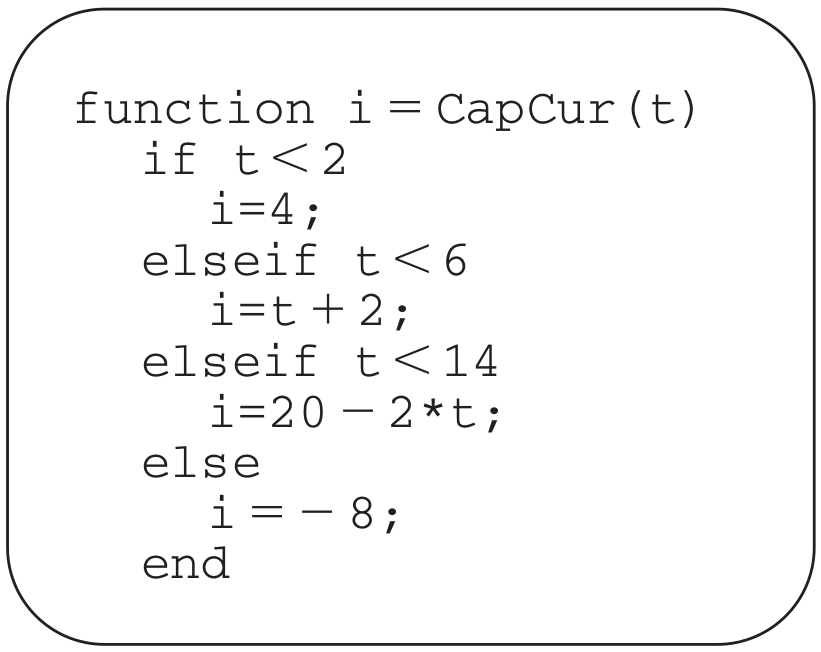
\includegraphics[width=3.8cm,height=2.5cm]{figure34.png} {.............}
    	  		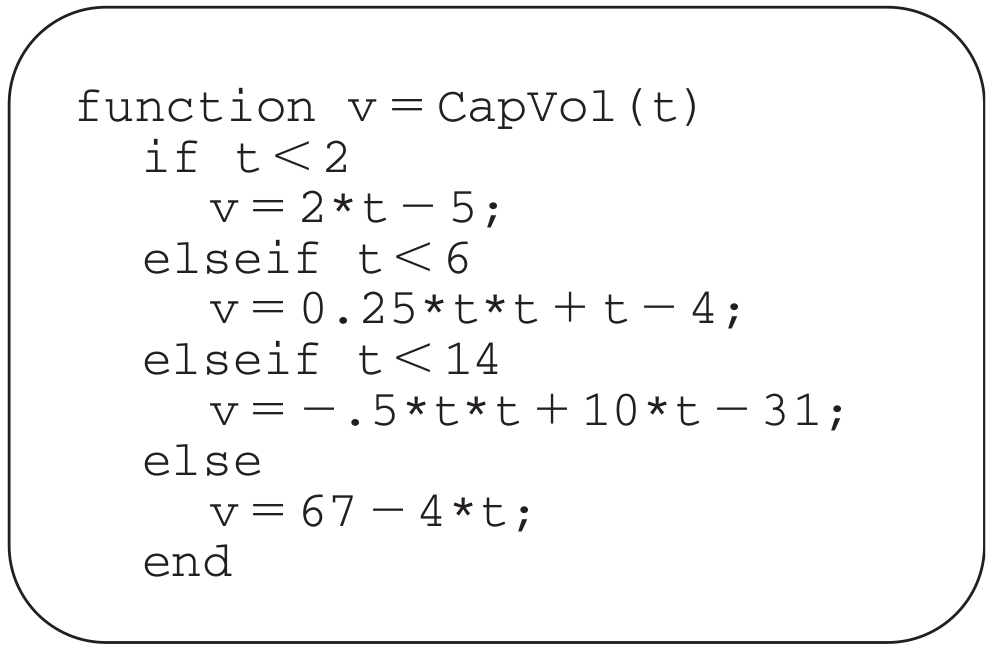
\includegraphics[width=3.8cm,height=2.5cm]{figure35.png}\\
    	  		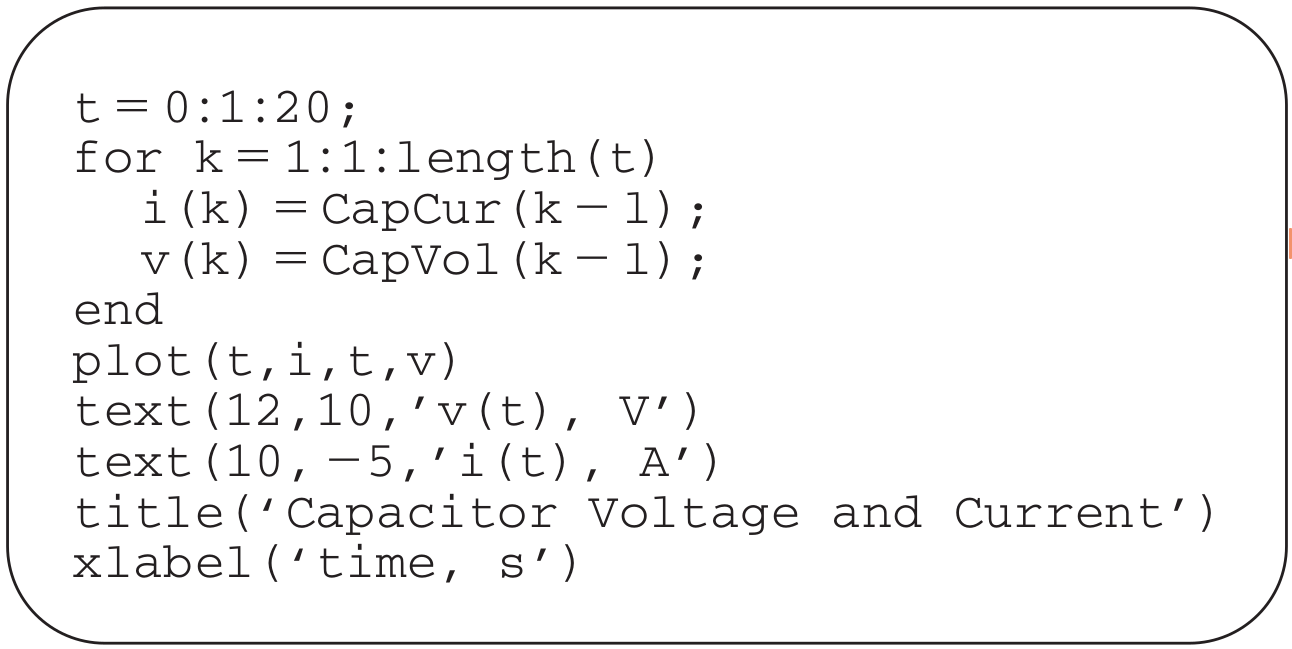
\includegraphics[width=3.8cm,height=2.5cm]{figure36.png}{.............}
    	  		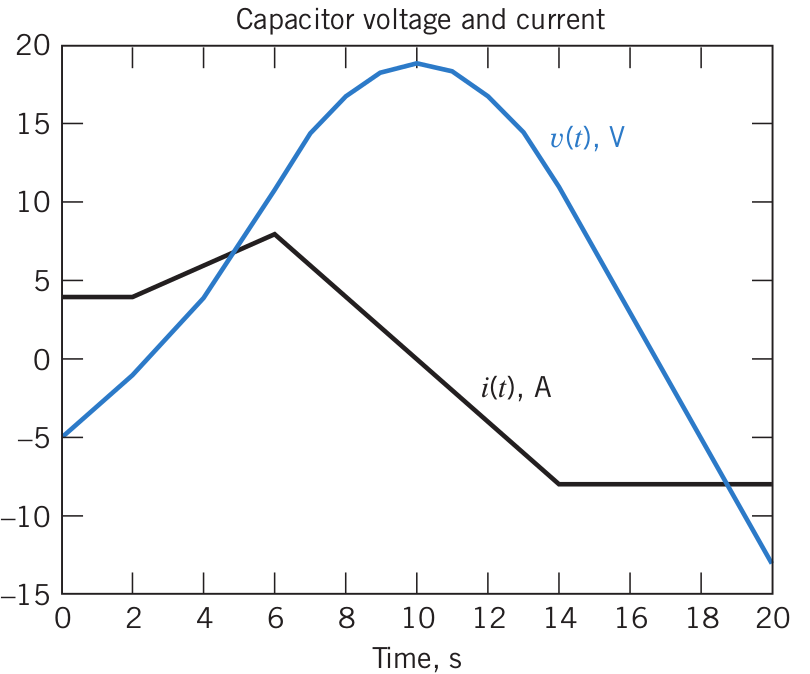
\includegraphics[width=3.8cm,height=2.5cm]{figure37.png}
		    \end{center}
		\end{column}
	

		
	
	
	\end{columns}\\
	
\end{tabular}
\end{frame}
	
	

\end{document} 

